% !TeX root = ../../main.tex
% Add the above to each chapter to make compiling the PDF easier in some editors.

\chapter{Setup and Implementation}\label{chapter:setup_and_implementation}

In this chapter, we will describe the setup for our environments with a description for each environment. The software that we will be using to run our experiments along with the implementation of the classes used to run the experiments.

\section{Overview}
Our approach is to run multiple experiments for different kinds of environments to test the agents in both normal and distributed training modes.

We have selected a couple of environments from different existing RL environments frameworks which is related to robotics simulations and continuous action spaces.

We have used Ray framework as our backend for the conducted experiments as it provides a reliable distributed training and scheduling algorithms along with \textit{tune} for hyperparameters tuning and grid searching to find the best configurations for all experiments, agents and environments (single, vectorized, and multi-agents).

% TODO: Remove
We have used Ray framework as our backend for the conducted experiments as it provides a reliable distributed training and scheduling algorithms along with \textit{tune} for hyperparameters tuning and grid searching to find the best configurations for all experiments, agents and environments (single, vectorized, and multi-agents).

\clearpage

\section{OpenAI: Reacher Environment}

Our first and baseline environment is \textit{Reacher Environment}~\ref{fig:openai_reacher}: A robotic arm consist of two linked joints places in a squared arena surrounding it along with a moving sphere (target). The goal of the robotics arm it to reach target sphere and maintain following the point until the end of the episode. 

\begin{figure}[h!]
    \begin{center}
            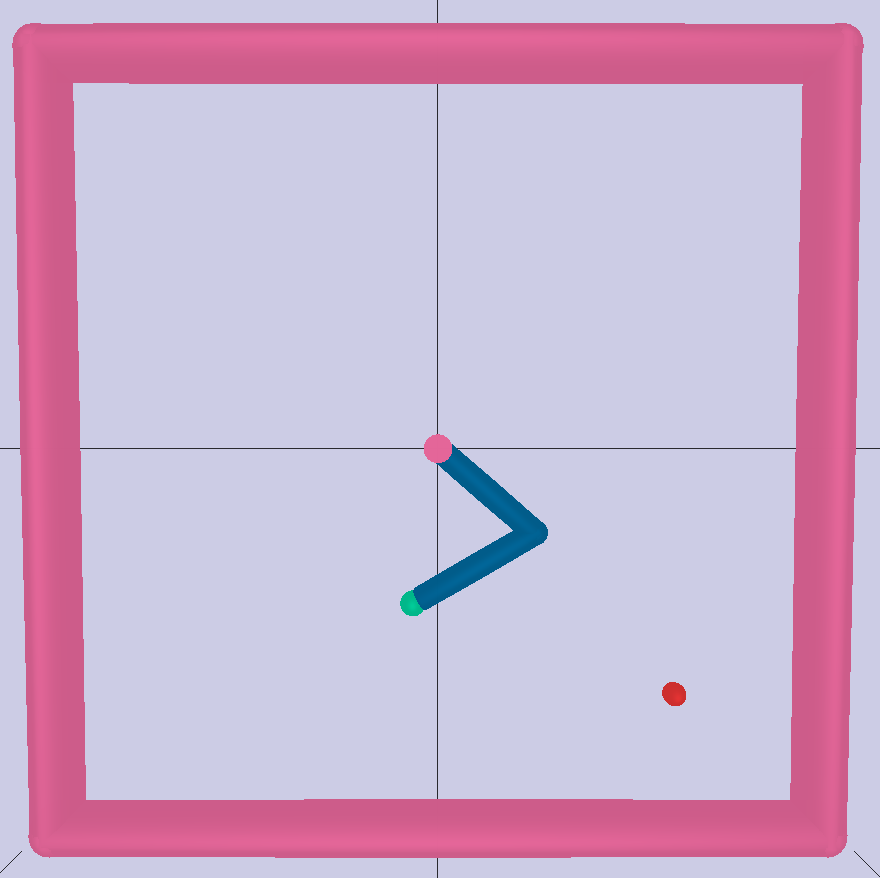
\includegraphics[width=.5\linewidth]{figures/envs/openai_reacher.png}
            \caption{OpenAI Reacher Environment}
            \label{fig:openai_reacher}
    \end{center}
\end{figure}

Environment Information:
The observation space consist of an array of 9 variables that includes [
    current target x position, 
    current target y position, 
    position vector 0 from arm to target,
    position vector 1 from arm to target,
    cosine of central joint current relative position,
    sine of central joint current relative position,
    gamma: elbow joint current relative position
    gamma dot: elbow joint current relative position
]

Action Space consist of two actions which are the forces applied to the torque of each joint